\documentclass{report}
\usepackage[parfill]{parskip}
\usepackage{todonotes}
\usepackage{hyperref}
\usepackage{amsmath}
\usepackage{wrapfig}
\usepackage{multicol}
\usepackage{graphicx}
\usepackage{fancyvrb}
\usepackage{minted}
\usepackage{textcomp}
\usepackage{bytefield}
\usepackage{longtable}
\usepackage{etoc}
\graphicspath{ {./img/} }
\begin{document}

\title{NEA: Font Rasterizer}
\author{Jake Irvine}


% THINGS LEFT TO DO:
%
% - expand docuemented design with flowcharts etc
% - finish testing & evaluation
% - spelling pass
% - cry????
% - replace std::abort with proper error checking
% - commenting pass on program

\maketitle
\chapter{Analysis}

Text is a key aspect of how we interact with machines. Virtually everything that
is done on a computer requires some form of reading on a screen. The program
that converts the binary text data to pixels on a screen is a `font engine' or
`font rasterizer'. These take some text or a single character and output a
texture (a collection of pixels) which will get copied into the screen buffer
(which is then copied onto the display itself to be shown to the user). There is
another component of font rendering, which arranges individual characters output
by a font rasterizer into words or paragraphs, called a layout engine.

Creating a full font engine is a very large task - the TrueType format (the
industry standard for font files) is a very large specification, and can be
further enhanced by vendor-specific extensions. For example, some fonts contain
small programs inside them that adjust the actual glyphs to better fit the pixel
grid of the screen. These are implemented in a custom virtual machine that is
very complex and time consuming to create. However, when rendering characters at
a large size, the impact of these features is far less, yet still comes at a
substantial performance cost.

To show a font on the screen, we must accomplish two tasks: \textbf{Parsing},
and \textbf{Rendering}. Parsing is the process of taking the raw font file
(which is just a set of bits) and converting it into data structures that make
it possible to access specific attributes or structures stored in the file. For
example, a key step in parsing the font will be to divide the file up into a
number of Glyph tables. Once this is done, the created data structures will be
passed to the renderer, which will turn these structures into a bitmap (set of
pixels) that is suitable for display on the screen.

The parser will take a TrueType font file and output the bezier curves of the
selected character, by reading the binary file. This is non-trivial, because the
TrueType format is relatively complex, and contains a lot of optional features
(which this project will largely ignore, unless I have time left over). I will
investigate parser-combinator systems and either use that or create my own
custom parser architecture.

TrueType fonts are composed of straight line segments and bezier curves. These
are primitives that are relatively easy to draw to the screen quickly, using
simple mathematical techniques. There are a number of additional options that
can be implemented in the renderer, such as anti-aliasing, which smooths the
sharp pixel edges of the shapes to make them appear smoother to the eye.

%\section{Project Scope}
%The TrueType format is very complex, and creating a full implementation is
%outside the scope of a NEA. For simplicity, I will focus on the most important
%part of the format: individual character glyphs. This avoids the need for
%parsing kerning data, ligatures, and other optional features that would be
%present in a full implementation. In addition, I will not implement the
%grid-fitting aspect of the specification, as this would require creating a
%virtual machine to run the instructions contained in the font.

%\todo{add to this later as i find more stuff i can't do}

\newpage
\section{Project Background}

\subsection{Domain Terminology}
\textbf{Font Family}: a collection of typefaces, at different weights, or styles
such as italics.
\\

\textbf{Typeface}: commonly referred to as a font, a typeface is a style of
lettering that can be displayed on the screen or in print.
\\

\textbf{Font}: an instance of a typeface at a specfic size.
\\

\textbf{Glyph}: the shape corresponding to a specific character in a specific
font.
\\

\textbf{TrueType}: TrueType is the industry standard for font files, and the
specific file format that is being targeted by this project. It contains all of
the data needed to describe a typeface (or sometimes multiple typefaces).
\\

\textbf{TTF file}: A file following the TrueType format.
\\

\textbf{Table}: a table in a TTF file is a section of data following a specfic
format that is indexed using the table directory at the start of the font file.
For example, the \texttt{glyf} table stores the actual glyph data of the font,
and the \texttt{cmap} table stores the mappings between character and glyph.
\\

\textbf{Anti-Aliasing}: the act of smoothing a line, curve or other bitmap with
lighter shades of it's colours to make it appear smoother to the viewier.

\begin{figure}[h]
  \centering
  
\includegraphics[width=0.4\textwidth]{aa}
  \caption{\textit{An anti-aliased line on the left, and a non-anti-aliased line
    on the right.}}
\end{figure}

\textbf{Bezier Curve}: A curve that is defined by a set of equation. The TTF
specification uses a variant of these called \textbf{Quadratic Bezier Curves},
which have a single control point. For more details see the section on Bezier
Curves below.
\\

\textbf{Raster Image}: A set of pixels that describe an image  

\subsection{Parsing}
As described above, parsing is the act of taking a text or binary sequence and
transforming it into data structures that can be used later. There are several
ways of doing this. Note that the process of parsing a font file is slightly
different to that of parsing a programming language or other free-form format.
Programming languages consist of a number of lines of code, whereas a font file
is highly structured, with every section of the file having a specific role
depending on it's position, (hereafter known as \textit{offset}).

\subsection{Bezier Curves}
\begin{wrapfigure}{r}{0.4\textwidth}
  \centering
  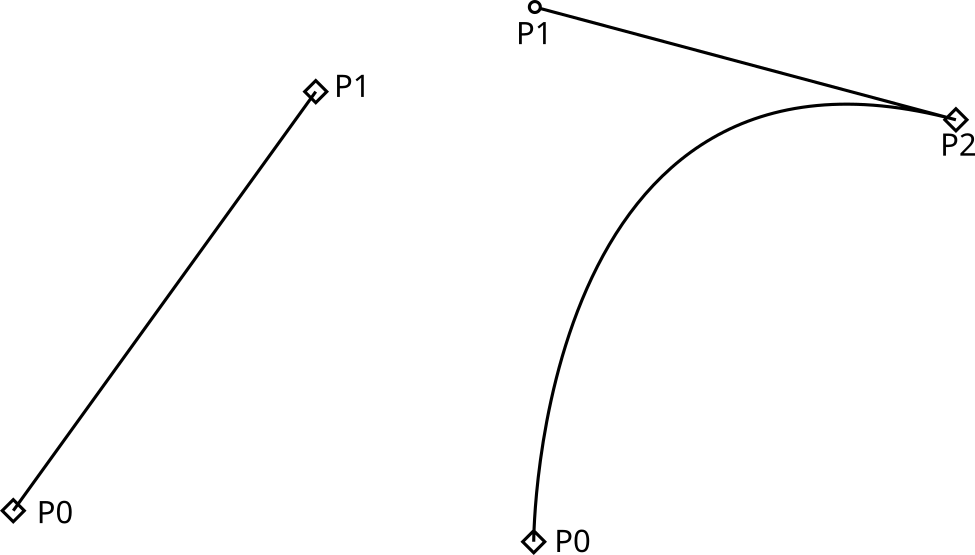
\includegraphics[width=0.4\textwidth]{bezier2img}
  \caption{\textit{A line segment and bezier curve, with control point}}
\end{wrapfigure}
Individual glyphs of a font are built up using \textit{outlines}, which are
themselves built of several segments of line and curve. More specifically, an
outline consists of a set of line segments and quadratic bezier curves, which
create a closed loop that forms all or part of the glyph. Luckily, both line
segments and bezier curves are fairly easy for computers to render, and have
been used in computer graphics since it's inception.

A quadratic bezier curve is described by the equation
\begin{equation*}
\mathbf{B}(t) = (1 - t)^2\mathbf{P}_0 +2(1 - t)t\mathbf{P}_1 + t^2\mathbf{P}_2
\end{equation*}
where $\mathbf{P}_0$, $\mathbf{P}_1$, $\mathbf{P}_2$ are the position vectors of
the 3 control points for the curve, as $t$ ranges from $0$ to $1$. We can draw
this in a similar way to how we draw line segments: for a sufficient sample rate
over $t$, we can evaluate $\mathbf{B}(t)$ and, rounding to the nearest pixel,
plot that point.
\begin{figure}[t]
\centering
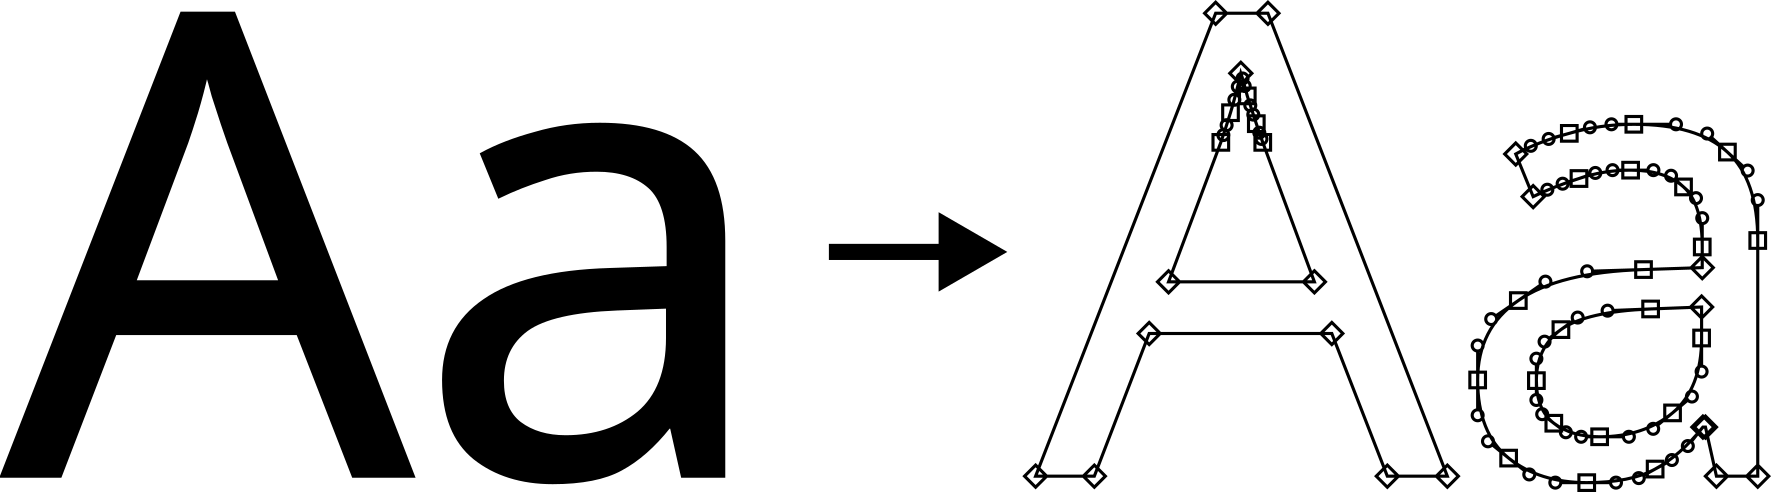
\includegraphics[width=0.6\textwidth]{outlineimg}
\caption{\textit{Letters are made up of line segments and bezier curves}}
\end{figure}
Similarly, we can describe a line segment (which is effectively a linear bezier
curve) using the following equation:
\begin{equation*}
  \mathbf{B}(t) = \mathbf{P}_0 + t(\mathbf{P}_1 - \mathbf{P}_0)
\end{equation*}
where $\mathbf{P}_0$, $\mathbf{P}_1$ are the two control points, the beginning
and end of the line segment. \todo{needs pictures}

\subsection{The Font Pipeline}

There are several stages involved in getting text to display on the screen.
First, the file containing the font is read. Often these are in a standard
folder, but all font systems support reading from arbutrary files. The file is
parsed (which means broken down into the data that's needed for the specific
task) and various tables in the font file are read. The glyph coordinate data
will then be parsed and read, usually into a cache.

Next is the hinting step. Because fonts are usually distributed as vectors, yet
they are being displayed on a fine pixel grid, naievely rendering them can
result in poor font quality. Hinting is an process of distorting the glyph to
better fit the pixel grid and size that it will be displayed on. A properly
hinted font contains a small program for each glyph, to be executced in a
virtual machine, that distorts the vector data to align with the pixel grid.
This is a very complex process that is responsible for most of the time
rendering the font.
\begin{wrapfigure}{r}{0.4\textwidth}
  \centering
  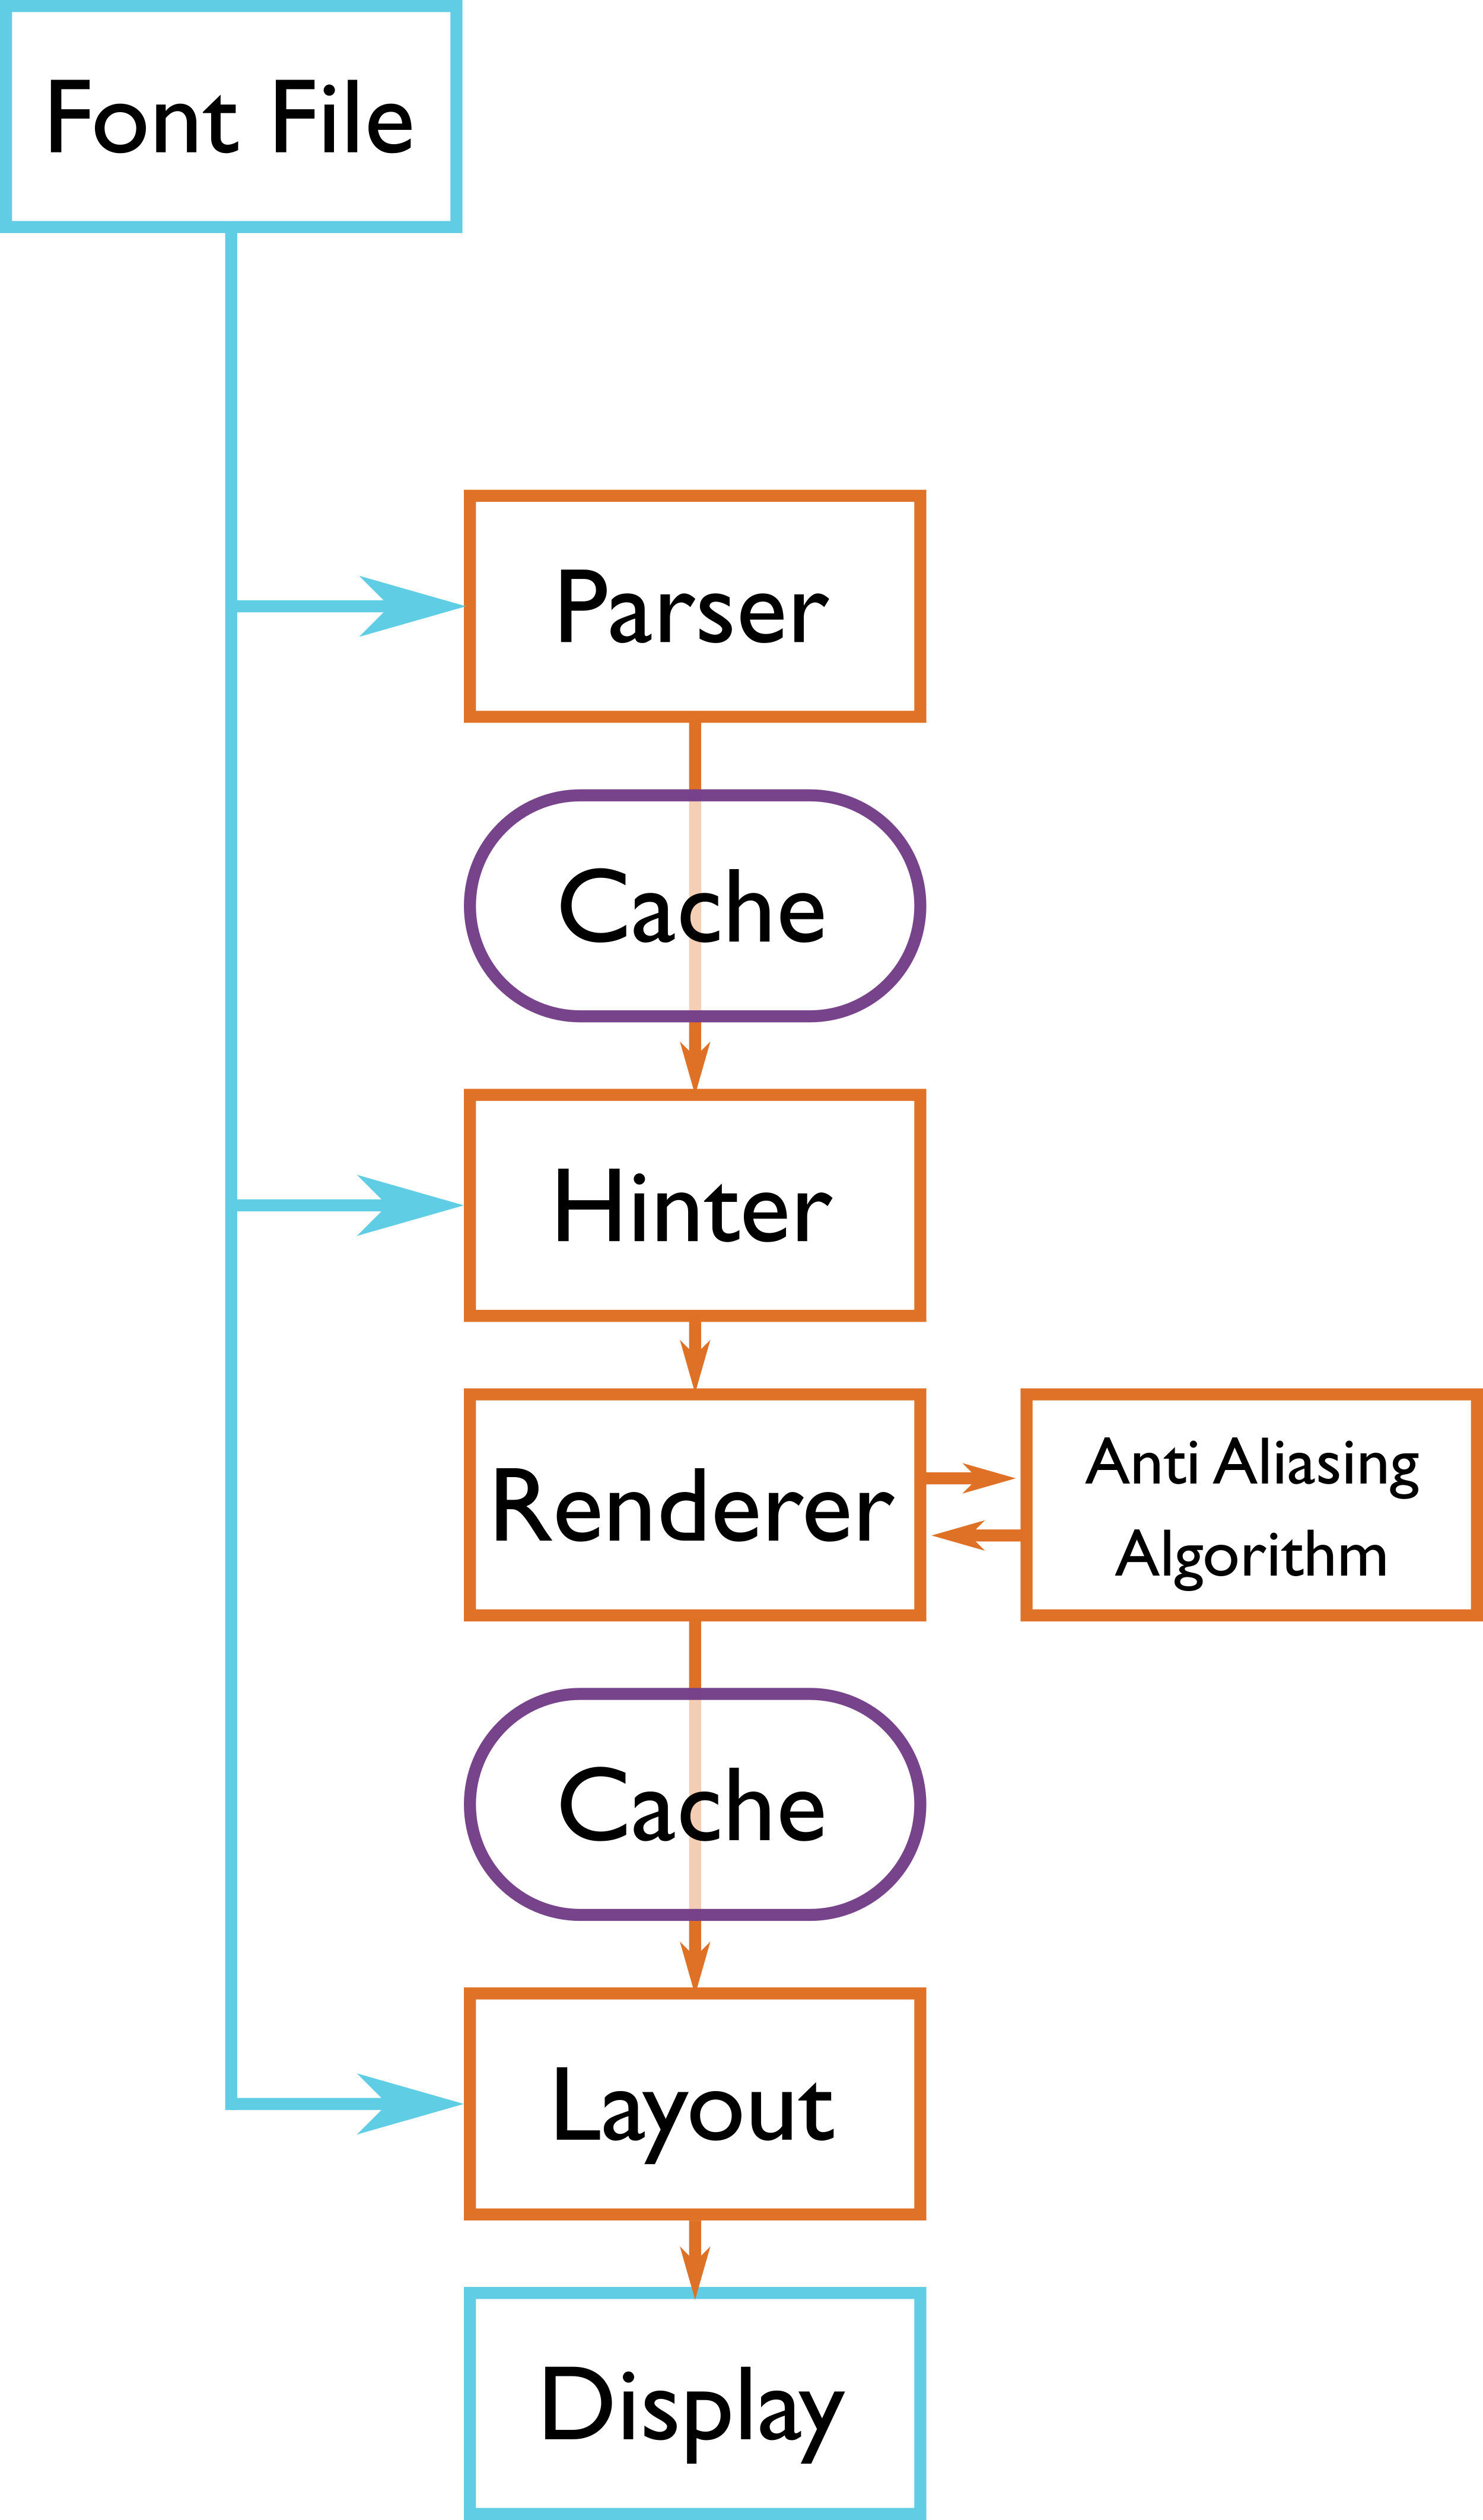
\includegraphics[width=0.4\textwidth]{fontpipelineimg}
\end{wrapfigure}

The hinted font is then rendered, taking the bezier curves of the font and
creating a raster image. This image is then anti-aliased, probably through
supersampling \todo{explain this more}, which is a process that turns a
black-and-white image to a greyscale one which looks sharper on the screen. Some
advanced anti-aliasing techniques take advantage of the RGB format of our
displays, to get a larger effective resolution to work with.

Finally, the anti-aliased image is displayed on the screen. The exact process
behind where it should be placed is handled by a layout engine, which is
responsible for forming individual glyphs into words and pages. A layout engine
still needs to reference the original font file, as kerning information which
dictates the individual spacing between characters is stored in a table there.

font file $\rightarrow$ parser $\rightarrow$ cache $\rightarrow$ hinting $\rightarrow$
rendering $\rightarrow$ anti-aliasing $\rightarrow$ layout


\subsection{The TrueType Format}
A TrueType font file is a binary file that contains all the data needed to
display a font on the screen. The format, initially codenamed `Bass', was
designed by Apple in the 1980s for Mac System 7, and has continued to evolve and
is now used by virtually every consumer operating system and font engine. The
full specification is available at
\url{https://developer.apple.com/fonts/TrueType-Reference-Manual/}, which will
be summarized here.
\begin{wrapfigure}{r}{0.4\textwidth}
  \centering
  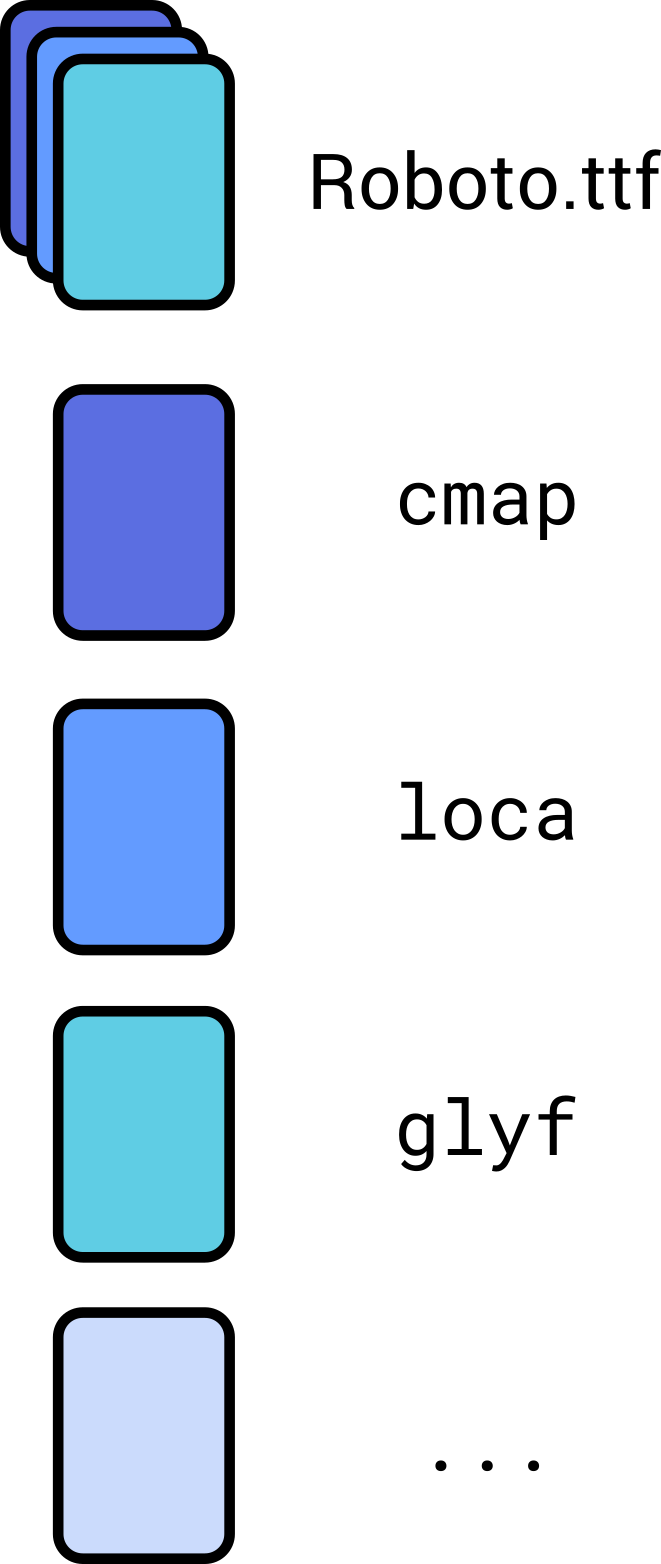
\includegraphics[width=0.2\textwidth]{breakdownimg}
\end{wrapfigure}
The format is a \textit{binary} file, which means that we look at the file in
terms of bytes, rather than in terms of characters and lines of text. The file
is composed of a number of \textit{tables}, which are analoguous to chapters of
a book. The file begins with the table directory, which is the table of contents
for these chapters -- it contains their titles, along with where in the file
they can be found. For example, the table directory may contain an entry for a
table called \texttt{glyf}, which points to the area of the file that stores the
glyph data for the font. 

There are several mandatory tables, as shown below. More tables may exist in the
file, but are optional, and may contain extensions to the format, or other data
such as raster images.
\begin{center}
  \begin{tabular}{ l | l }
    
    Name & Function \\
    \hline
    \texttt{cmap} & Maps between characters and glyphs \\
    \texttt{glyf} & Stores the actual glyph data \\
    \texttt{head} & Font header, contains various data involved in the rest of the font \\
    \texttt{hhea} & Secondary header containing specifics of horizontal font layout \\
    \texttt{hmtx} & Data on the metrics of fonts when layed out horizontally \\
    \texttt{loca} & Indexes glyph IDs to offsets in the file \\
    \texttt{maxp} & Contains the maximum quantities of various features of the font \\
    \texttt{name} & Contains the name of the font \\
    \texttt{post} & Data for printing fonts \\
  \end{tabular}
\end{center}

The tables of relevance to this project are \texttt{head}, \texttt{loca},
\texttt{cmap}, and \texttt{glyf}. A detailed explanation of table data
structures can be found in the TrueType specification; a simplified version of
the \texttt{glyf} table is shown below:

The \texttt{glyf} table consists of a number of glyph data structures. Each data
structure is either a simple or compound glyph, and is of the form

\begin{bytefield}[bitwidth=2.2em]{16}
  \bitheader{0-15} \\
  \begin{rightwordgroup}{Glyph header}
    \wordbox{1}{numberOfContours} \\
    \bitbox{16}{xMin} \\
    \bitbox{16}{xMax} \\
    \bitbox{16}{yMin} \\
    \bitbox{16}{yMax} 
  \end{rightwordgroup} \\

  \wordbox{3}{Either a simple glyph data structure, or a compound glyph data
    structure, dependent on the value of \texttt{numberOfContours}.}
\end{bytefield}
\\

\begin{bytefield}[bitwidth=2.2em]{16}
  \bitbox{16}{\textbf{Simple Glyph Data}} \\
  \bitheader{0-15} \\
  \wordbox{2}{Array of glyph contour endpoints, one word wide,
    \texttt{numberOfContours} long.} \\
  \wordbox{1}{instructionLength} \\
  \bitbox{8}{Instruction 1} & \bitbox{8}{Instruction 2} \\
  \bitbox{8}{Instruction 3} & \bitbox{8}{...} \\
  \bitbox{8}{...} & \bitbox{8}{Instruction $n$} \\
  \wordbox[tlr]{3}{Array of flags, length can be determined from the final
    endpoint index} \\
  \bitbox[l]{8} {Example:} & \bitbox{1}{C} & \bitbox{1}{xSh} & \bitbox{1}{ySh} &
  \bitbox{1}{R} & \bitbox{1}{xR} & \bitbox{1}{yR} & \bitbox{2}{Reserved} \\
  \wordbox[blr]{1}{}\\
  \wordbox{2}{Array of deltaX}\\
  \wordbox{2}{Array of deltaY}\\

\end{bytefield}

\textit{Note: Compound glyph tables are outside of the scope of this project.}
\\
\\

To turn a character into a set of points, we must first lookup the character in
the \texttt{cmap} table. This will give us a glyph index, which we can index
into the \texttt{loca} table to get a glyph offset and length. Finally, we can
use the offset and length to find the appropriate section of the \texttt{glyf}
table, and get the glyph data itself.

\subsection{Hinting}

The TrueType format provides support for font hinting, which is a set of small
adjustments to the generated outline before it is displayed on the screen to
make it better fit the pixel grid. These are implemented through a virtual
machine, which runs a set of instructions that alter the font metrics and points
at runtime.   

\section{Existing Solutions}

Since we can see text on a screen, there are clearly several existing solutions
to font rasterization. A few prominent examples are outlined below.



\subsection{freetype}
Freetype is a free, open source font engine that is used in many large software
projects, such as GNU/Linux, iOS and Postscript. It supports the vast majority
of font features and formats, including little-used ones such as .FON files and
X11 PCF fonts. However, due to this, it is very large, and rather slow.

Advantages:
\begin{itemize}
\item{Can handle virtually any font format you may need.}
\item{A full implementation of the TrueType specification, meaning it supports
    all of the features of the specification, as well as a number of vendor
    specific extensions.}
\item{Will run on a wide variety of systems, including the 16-bit Atari and
    Amiga computers.}
\item{Supports a wide range of character encodings, including the full unicode
    range of encodings, such as UTF-8 and UTF-16.}
\end{itemize}

Disadvantages:
\begin{itemize}
\item{Slow, due to it's support of the full specification.}
\item{Has a large memory footprint, meaning there is less space available for
    other programs.}
\item{Has a relatively complex API, that can be harder to integrate into
    applications already using a different font engine.}
\item{It does not handle complex layouts, which may be useful for some users.}
\end{itemize}

\subsection{SDL\_ttf}
SDL\_ttf is a ready to use library for rendering fonts to a texture using the
SDL graphics library. Internally, it uses the freetype library as discussed above.

Advantages:
\begin{itemize}
\item{Simple to integrate into (SDL) applications.}
\item{Uses the freetype backend, which supports a wide range of font features.}
\item{Can be compiled for any platform, due to the fact that it's written
    using crossplatform libraries and C++.}    
\end{itemize}

Disadvantages:
\begin{itemize}
\item{Slower than using freetype alone, because it adds SDL bindings on top of
    it.}
\item{Can only render on the CPU, failing to take advantage of any GPU that may
    be present.}
\item{Since it uses SDL for rendering, it can be quite hard to use with a non
    SDL project.}
\item{Due to it's simple API, it fails to expose many advanced features of
    freetype, that might be useful to a client.}
\end{itemize}

\subsection{Quartz}
Quartz is the font renderer used on MacOS and iOS devices, for almost all
software. It uses subpixel positioning, which means each glyph doesn't have to
be aligned with the pixel grid, instead being allowed to be anywhere between
pixels, using subpixel rendering and anti-aliasing to properly handle this
case.

Whilst this can result in clearer display at high dpi resolutions, (such as
Apple's retina displays), at lower dpi monitors or smaller font sizes it can
result in harder to read text.

Advantages:
\begin{itemize}
  \item{Provides the closest similarity to printed text when viewed on high DPI
      displays. }
  \item{Is included by default with MacOS and iOS}
\end{itemize}

Disadvantages:
\begin{itemize}
\item{Will only run on MacOS / iOS devices}
\item{The subpixel grid can make fonts look blurry at low DPI monitors.}
\end{itemize}

\section{User Feedback}

I consulted with a potential user of my project, to assist in determining what
my priorities should be. They use computers for programming, revision, and
entertainment, so they spend a lot of time looking at computer-generated text.
They also program GUI based applications that need to display text on the
screen, so they are the target user for this system.
Their responses are shown below in italics:

Do you notice the speed of font rendering on your computer?

\textit{Usually no, as most programs render at small resolutions. However, some
  programs such as my PDF viewer (Zathura) take a very long time rendering fonts
  when zoomed way in.}

Do you notice the quality of font rendering on your computer?

\textit{Usually it is perfectly fine, but occasionally kerning issues.}

What features would you want from a typeface rendering system?

\textit{Fast and accurate rendering, the ability to output SVGs, support for
  common modern fonts, a good API for integrating into other libraries or
  programs, compatibility with SDL/OpenGL libraries, debugging tools for viewing
  path tracing.}

Is speed a concern in a font renderer?

\textit{Definitely. As soon as it becomes less-than-instant it becomes a
  productivity bottleneck and can make navigating an operating system
  frustrating.}

Would you rather have increased speed of a font rendering system, or support of more advanced typographical features?

\textit{A balance of both. Performance should be considered, but not over every other feature.}

I used these responses along with my analysis above to determine what, and what
priority, I should give to my objectives below. 

\section{Project Objectives}
\begin{center}
  \begin{longtable}{c|c|p{3cm}|p{6.5cm}}
    \# & \textbf{Priority} & \textbf{Description} & \textbf{Reasoning} \\
    \hline
    1 & High & The system will accept correctly formed TTF files as input. & The TrueType format has been chosen because it is the industry standard, and almost every font available today can be obtained in TTF format. It also has a rigid specification, and support from other font rendering systems. \\
    \hline
    2 & Medium & The system will reject files that do not exist, or are not correctly formed TTF files. & Cleanly handling errors is important for usability and stability. \\
    \hline
    3 & High & The system will correctly parse the tables \texttt{head}, \texttt{cmap}, \texttt{loca}, and \texttt{glyf} to read the font. & This is critical functionality, required for any displaying of any character from the font. \\
    \hline
    4 & Low & The system will output information about the tables on stdout. & This would be beneficial for both debugging purposes and to demonstrate how the internals of a font work. \\
    \hline
    5 & High & The parser section of the system will output bezier curves that
               can be sent to the renderer to display the font, or exposed via
               an API for use in some other application. & Critical
                                                           functionality that is
                                                           required to display
                                                           any fonts at all. \\
    \hline
    6 & High & The system will accept an ASCII character to be the glyph to be
               parsed and eventually displayed. & This will be part of the
                                                  demonstration of my renderer,
                                                  which is additionally useful
                                                  for testing \\
    \hline
    7 & Medium & The system will render fonts at large point-sizes quickly.
                                                  & This is a key factor
                                                    identified by the user
                                                    consultation, as they said
                                                    that their current solution
                                                    was unacceptably slow. \\
    \hline
    8 & Medium & The rendering subsystem will render the curves given to it by
                 the parser at a high readability and with anti-aliasing.
                                                  & The readability of fonts is
                                                    an area that is already
                                                    covered well by existing
                                                    solutions as discussed
                                                    above, but simple
                                                    readability improvements
                                                    such as anti-aliasing are
                                                    relatively simple to
                                                    implement and make a
                                                    large difference to the final
                                                    output. \\
    \hline
    9 & Low & The system will export font outlines to SVG. & This is another
                                                            feature identified
                                                            in the user
                                                            consultation, but
                                                            due to time
                                                            constraints I may
                                                            not be able to
                                                            implement it.
                                                            However, I will try
                                                            to design the
                                                            program in such a
                                                            way that adding it
                                                            later will be simple. 

  \end{longtable}
\end{center}


\chapter{Design}
\section{High Level Design}

\begin{wrapfigure}{r}{0.5\textwidth}
  \centering
  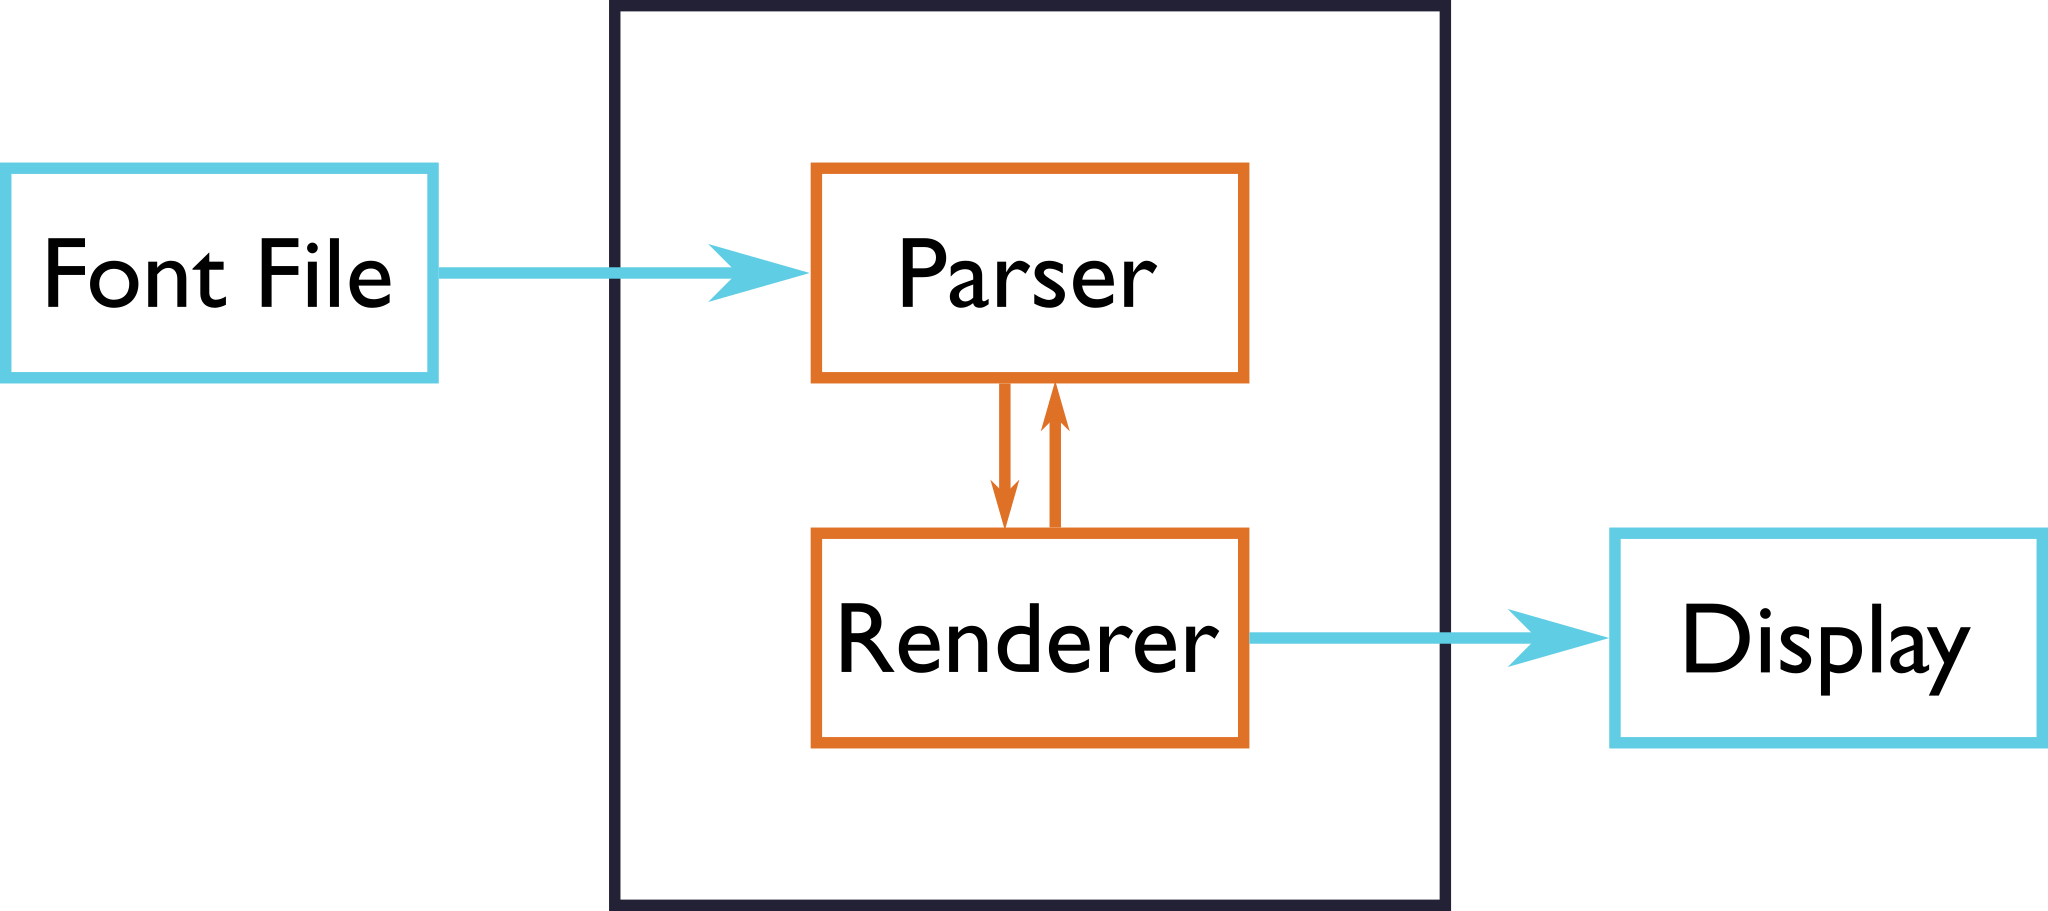
\includegraphics[width=0.5\textwidth]{design/highlevelout}
\end{wrapfigure}

The task has 2 clear subdivisions:
\begin{enumerate}
\item{Parsing the specified font file.}
\item{Displaying the parsed bezier curves on the screen.}
\end{enumerate}


I anticipate task 1 being the hardest, because the TrueType format is very
complex and requires sophisticated parsing to extract the data needed. In
contrast, rendering bezier curves to the screen is a task is moderately simple,
as the bezier curve is used frequently in computer graphics applications.

I have selected C++ as the programming language for this project, because I am
familiar with it, and whilst it supports high-level concepts such as
object-oriented programming, it is easy to modify variables at the byte level,
which is needed for some parsing stages. I use the cmake build system, because
it is integrated well into my tools (Intellij CLion). This makes compiling large
C++ programs easier, and means I only need to recompile sections of my program
that change, which will speed up developement times.

I have also decided to use the SDL 2D graphics library to draw the curves and display the
resulting image on the screen. I have used this library before, and it is both
fast (it can be used in a mode that is GPU-accelerated) and easy to use. In
addition, it means my library can be very easily integrated into any other SDL
application. I will also use an additional library, \texttt{sdl\_gfx} to assist
with rendering anti-aliased curves. Note that I am not using the standard
version of the library -- instead, I am using a slightly modified version that
supports rendering anti-aliased bezier curves.

%I will program in C++, using the cmake build system, and use the SDL graphics
%library to display the rendered characters to the screen. Finally, I will use a
%slightly modified version of \texttt{sdl\_gfx} to make rendering the characters easier. 

\subsection{The Parser}
The parser needs to take the filename of a font, and by examining the associated
file, read various data about the font. The following is a loose list of the
data needed; other data may be needed to properly parse this, or for other
purposes.

\begin{enumerate}
  \item{The \texttt{head} table, which contains information about the rest of
      the file}
  \item{The \texttt{cmap} table, which contains the mapping between character
      and glyph index}
  \item{The \texttt{loca} table, which maps glyph indices to offsets from the
      start of the \texttt{glyf} table}
  \item{The individual glyph data, which requires the above data points to
      find in the file}
  \item{Various font metrics, contained in various tables around the font file}
\end{enumerate}

At the very beginning of the file is the table directory, which contains the
locations and length of all the font tables. Parsing this allows us to look up
the locations of the rest of the data in the file. Next we will examine the
\texttt{head} table to store important metrics that will be used elsewhere in
the file.

At this point, the program will prompt the user for the character that they
would like displayed. This character will be looked up in the \texttt{cmap}
table, to get a glyph index, and then the \texttt{loca} table, to convert the
index into a glyph offset and length.

Finally, we lookup the glyph in the \texttt{glyf} table, and store the entire
glyph data structure. This is quite complex to parse, and will have it's own
section of the program specifically. Parsing this will result in a list of
bezier curves to be rendered, which is then passed to the renderer. 

\subsubsection{The \texttt{Font} class}
A key data structure in this project will be the \texttt{Font} class. This is a
large structure that represents a specific font. We create one at the start of
our program, and gradually fill it in over the course of parsing the font. 

\begin{center}
  \begin{tabular}{|p{7.5cm}|c|c|}
    \hline
    \multicolumn{3}{|c|}{The \texttt{Font} class} \\
    \hline
    \textbf{Type} & \textbf{Name} & \textbf{Access} \\
    \hline
    \texttt{Glyph} & glyph & public \\
    \hline
    \texttt{std::string} & filename & private \\
    \hline
    \texttt{Header} & header & private \\
    \hline
    \texttt{HEADTable} & head & private \\
    \hline
    \texttt{CMAPTable} & cmap & private \\
    \hline
    \texttt{std::vector<uint8\_t>*} & data & private \\
    \hline
    \texttt{int} & fileLength & private \\
    \hline
    \texttt{char} & characterToGet & private \\
    \hline
    \texttt{uint32\_t} & glyphOffset & private \\
    \hline
    \texttt{uint32\_t} & glyphLength & private \\
    \hline
    \hline
    \textbf{Signature} & \textbf{Returns} & \textbf{Access} \\
    \hline
    \texttt{Font()} & Font & public \\
    \hline
    \texttt{Font(std::string filename, char characterToGet)} & Font & public \\
    \hline
    \texttt{readFont(std::string filename)} & void & private \\
    \hline
  \end{tabular}
\end{center}

The most important section of this class is the \texttt{readFont} method. It is
called in the constructor of the font, and does the following things:

\begin{enumerate}
\item Opens the file speficied by \texttt{filename}.
\item Reads that file into the \texttt{data} variable in memory.
\item Parses the header of the font to get the offsets of the tables.
\item Parses the HEAD table into the the \texttt{head} variable.
\item Parses the CMAP table into the \texttt{cmap} variable.
\item Uses the \texttt{cmap} table to get the glyph index of the requested glyph.
\item Looks up this glyph index in the \texttt{loca} table.
\item Parses the glyph using that information. 
\end{enumerate}

This prepares the font to be passed to the renderer, where the public member
\texttt{glyph} will be read by the renderer itself to draw the font to the screen.

\subsubsection{Parsing Fonts}

The TTF specification uses a number of different types of data, which must be
parsed from a series of bytes. My project has a utility module that contains
various functions to take a data array and an offset, and can return a requested
data type from that data. For example, \texttt{parse16} will return a signed 16-bit
integer parsed from the bytes after the offset given. These functions are used
throughout the project, and the util module is included in nearly every file of
the parsing system.

\subsubsection{The Glyph Table}

The core algorithm of the parsing section is the glyph parser. To save space,
data in the glyph itself is not repeated, instead a special flag is set to tell
the parser to repeat this data again. In addition, we must calculate when to
switch from parsing x values to parsing y values, which requires special
calculations to do. The algorithm in pseudocode is as follows:

\begin{Verbatim}[numbers=left]
Glyph::parse(data, offset, length):
  numberOfContours = parse an unsigned 16bit integer at (offset)
  xMin = parse an unsigned 16bit integer at (offset+2)
  yMin = parse an unsigned 16bit integer at (offset+4)
  xMax = parse an unsigned 16bit integer at (offset+6)
  yMax = parse an unsigned 16bit integer at (offset+8)

  if numberOfContours < 0:
    abort() (compound glyphs are outside the scope of the program)

  endPointsOfContours = empty vector
  for (i = 0; i < numberOfContours; i++):
    parse a 16bit integer at (offset+10+i*2) and append it to   \
    endPointsOfContours

  instructionOffset = offset+10+numberOfContours*2
  instructionLength = parse an unsigned 16bit integer at
                      (instructionOffset)

  dataOffset = instructionOffset + instructionLength
  currentOffset = dataOffset
  
  totalPoints = the last value of endPointsOfContours

  flags = empty vector
  xDeltas = empty vector
  yDeltas = empty vector

  currentOffset += 2
  
  while numberOfPoints < totalPoints:
    construct a PointFlag at the currentOffset and append it to  \
    the flags vector
    numberOfPoints++
    currentOffset++

  currentOffset--

  for each flag in flags:
    xDelta = 0
    if xShortVector is set in flag:
      currentOffset++
      xDelta = parse an unsigned 8bit integer at (currentOffset)
      if sign is not set in flag:
        xDelta = -xDelta
    else:
      if xSame is not set in flag:
        currentOffset++
        xDelta = parse a signed 16bit integer at (currentOffset)
        currentOffset++
      else: (if xSame is set)
        xDelta = 0 
    append xDelta to xDeltas

  repeat the above loop for the yDeltas

  for each i in range(length(xDeltas)):
    point = (xDelta, yDelta, flag)
    append point to points

  return points
\end{Verbatim}

\todo{EXPLAIN THIS PROPERLY}

\subsection{Rendering}

The rendering system is comparitively much simpler. We take the points array
returned by the algorithm above, and draw it to the screen. To make this process
simpler, we use a slightly modified version of the \texttt{sdl\_gfx} library.
This library has been modified to allow for anti-aliased bezier curves, which
previously the library did not support. 

First, we iterate through the list of points to convert all of the delta values
into absolute coordinates. During this process, we also insert phantom points
between two off-curve points, to allow the drawing routine to look at the points
in sets of two or three. Finally, we add the first point again at the end of the
loop, to ensure that the loop gets closed.

Now that we have prepared our final list of points, we iterate through each
point, drawing either a line or a bezier curve (using the \texttt{sdl\_gfx}
library functions) as required. These are drawn onto the back framebuffer, which
is then made the active framebuffer (and displayed on the screen) with the call
to \texttt{SDL\_RenderPresent} in \texttt{main()}.

\chapter{Technical Solution}

\localtableofcontents

\section{cmakelists.txt}
\inputminted[linenos, frame=lines, framesep=2mm, breaklines]{cmake}{/home/jake/TTFParser/CMakeLists.txt}

\section{main.cpp}
\inputminted[linenos, frame=lines, framesep=2mm, breaklines, tabsize=4]{cpp}{/home/jake/TTFParser/src/main.cpp}

\section{util.h}
\inputminted[linenos, frame=lines, framesep=2mm, breaklines,
tabsize=4]{cpp}{/home/jake/TTFParser/include/util.h}
\section{util.cpp}
\inputminted[linenos, frame=lines, framesep=2mm, breaklines,
tabsize=4]{cpp}{/home/jake/TTFParser/src/util.cpp}
\section{Font.h}
\inputminted[linenos, frame=lines, framesep=2mm, breaklines, tabsize=4]{cpp}{/home/jake/TTFParser/include/Font.h}
\section{Font.cpp}
\inputminted[linenos, frame=lines, framesep=2mm, breaklines,
tabsize=4]{cpp}{/home/jake/TTFParser/src/Font.cpp}

\section{Header.h}
\inputminted[linenos, frame=lines, framesep=2mm, breaklines,
tabsize=4]{cpp}{/home/jake/TTFParser/include/Header.h}

\section{Header.cpp}
\inputminted[linenos, frame=lines, framesep=2mm, breaklines,
tabsize=4]{cpp}{/home/jake/TTFParser/src/Header.cpp}

\section{CMAPTable.h}
\inputminted[linenos, frame=lines, framesep=2mm, breaklines,
tabsize=4]{cpp}{/home/jake/TTFParser/include/CMAPTable.h}

\section{CMAPTable.cpp}
\inputminted[linenos, frame=lines, framesep=2mm, breaklines,
tabsize=4]{cpp}{/home/jake/TTFParser/src/CMAPTable.cpp}

\section{HEADTable.h}
\inputminted[linenos, frame=lines, framesep=2mm, breaklines,
tabsize=4]{cpp}{/home/jake/TTFParser/include/HEADTable.h}

\section{HEADTable.cpp}
\inputminted[linenos, frame=lines, framesep=2mm, breaklines,
tabsize=4]{cpp}{/home/jake/TTFParser/src/HEADTable.cpp}

\section{Glyph.h}
\inputminted[linenos, frame=lines, framesep=2mm, breaklines,
tabsize=4]{cpp}{/home/jake/TTFParser/include/Glyph.h}

\section{Glyph.cpp}
\inputminted[linenos, frame=lines, framesep=2mm, breaklines,
tabsize=4]{cpp}{/home/jake/TTFParser/src/Glyph.cpp}

\section{Point.h}
\inputminted[linenos, frame=lines, framesep=2mm, breaklines,
tabsize=4]{cpp}{/home/jake/TTFParser/include/Point.h}

\section{Point.cpp}
\inputminted[linenos, frame=lines, framesep=2mm, breaklines,
tabsize=4]{cpp}{/home/jake/TTFParser/src/Point.cpp}

\section{PointFlag.h}
\inputminted[linenos, frame=lines, framesep=2mm, breaklines,
tabsize=4]{cpp}{/home/jake/TTFParser/include/PointFlag.h}
\section{PointFlag.cpp}
\inputminted[linenos, frame=lines, framesep=2mm, breaklines,
tabsize=4]{cpp}{/home/jake/TTFParser/src/PointFlag.cpp}
\section{TableHeader.h}
  \inputminted[linenos, frame=lines, framesep=2mm, breaklines,
  tabsize=4]{cpp}{/home/jake/TTFParser/include/TableHeader.h}
\section{TableHeader.cpp}
\inputminted[linenos, frame=lines, framesep=2mm, breaklines,
tabsize=4]{cpp}{/home/jake/TTFParser/src/TableHeader.cpp}

\section{log.h}
\inputminted[linenos, frame=lines, framesep=2mm, breaklines,
tabsize=4]{cpp}{/home/jake/TTFParser/include/log.h}

\section{log.cpp}
\inputminted[linenos, frame=lines, framesep=2mm, breaklines,
tabsize=4]{cpp}{/home/jake/TTFParser/src/log.cpp}


\chapter{Testing}

To test the project I used a number of different methods to test my code. During
the intial programming of the technical solution, I used a debugger to directly
step through the code, along with directly modifying the code to print debugging
information to the console. I also compared the values various parts of my
program produced with the values produced by Freetype, another font rendering
system described in the analysis section. Once the solution had been completed,
I tested by running the code with a variety of inputs, and visually comparing
the output to reference images.

\subsection{Debugging}
For most of the programming work on this project I used the IDE CLion.
\begin{center}
  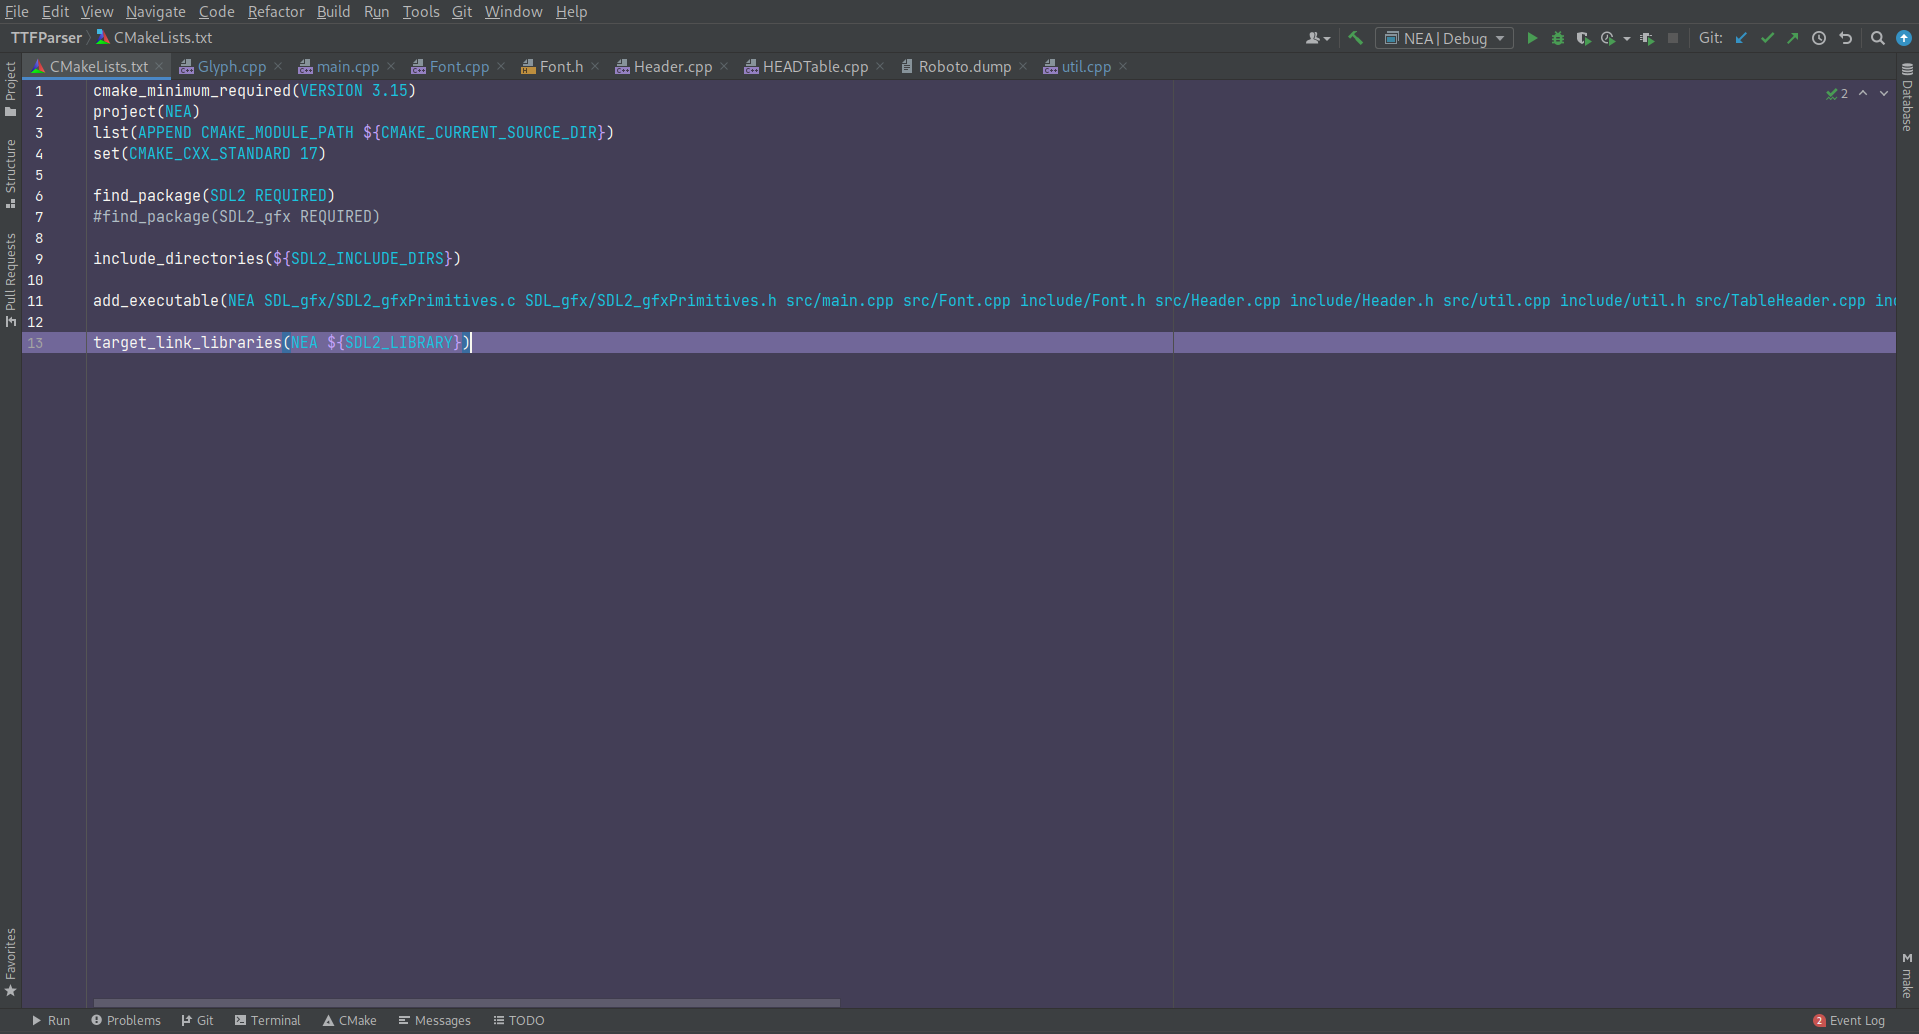
\includegraphics[width=12cm]{ide}
  \end{center}
This is a highly sophisticated IDE that has many features that make developing
C++ programs easier. The most useful of these is the visual debugger. This
allows you to pause the program at any point, inspect and change the values of
local and global variables, and generally get more of an understanding of how
your program works.

I used debugging extensively throughout this project, for a number of purposes.
When I was first writing the various modules, I used debugging as a basic sanity
check that my code was running. Because I was using C++, an unsafe language, I
was directly manipulating pointers at times, which meant that a Segmentation
Fault (when a program tries to read from invalid memory) could occur. The
debugger catches this, and I can see the exact line at which the segfault
occurs, which makes it significantly easier to identify and resolve the issue.

\begin{figure}[h]
  \centering
  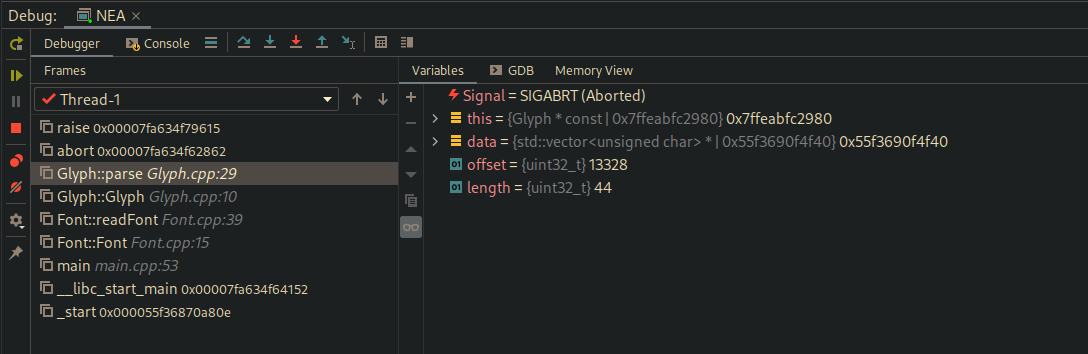
\includegraphics[width=12cm]{debugging1}
  \caption{\textit{My debugger after a segmentation fault has occured}}
\end{figure}


\subsection{Unit Testing}

Unit testing is the act of testing a program one unit at a time, so that you can
be sure that if all units are working as expected, then hopefully the entire
program is working as expected. To accomplish this I created my own sections of
TTF files that would test specific areas of the program, and ran it explicitly
with those files. This meant that if something broke, I could run my tests to
determine which area the problem is, complementing my other debugging using a
manual debugger.

\section{Testing the final program}
To test the final program, I used a number of methods. First, I simply observed
the output, to check that it resembled the font that I was giving it. I then put
the program through a set of tests that measured it's speed, as well as
comparing it's output to inkscape, which internally uses freetype as it's font
renderer. Finally, I tested it with fonts other than that of Roboto, which I had
been using to test the font whilst I was developing the system.

\subsection{Sample Outputs}
\begin{figure}[h]
  \centering
  \begin{minipage}{.5\textwidth}
    \centering
    
\includegraphics[width=.45\textwidth]{sample1}
    
\includegraphics[width=.45\textwidth]{sample3}
  \end{minipage}
  \begin{minipage}{.5\textwidth}
    \centering
    
\includegraphics[width=.45\textwidth]{sample2}
    
\includegraphics[width=.45\textwidth]{sample4}
  \end{minipage}
\end{figure}

The above samples are from my program, running with the font Roboto.ttf. The
program supports all alphanumeric characters, along with most of the rest of the
displayable ASCII range. The only notable exclusion is the semicolon (`;') which
is a compound glyph, reusing the glyph for full stop. The parsing of these
proved too complicated to implement in the time given, but the architecture of the program
means that it could be easily added in later.

\subsection{Objective 1: The system will accept correctly formed TTF files as
  input.}
I tested this by running my program with several correctly formed TTF files:
Roboto, Roboto Italic, Noto Sans, and Hack Mono. The first three files loaded
correctly into my program, whereas Hack Mono resulted in an error. Further
investigation revealed that Hack Mono used an advanced feature of the
\texttt{loca} table that my parser did not support. As a result of this testing,
I added code to safely handle this error, so that files containing unsupported
features are rejected with a descriptive error message rather than the program simply crashing.

\subsection{Objective 2: The system will reject files that do not exist, or are
  not correctly formed TTF files.}

To test this, I inputted the filenames of nonexistent files and files that are
not TTF files into the generator. I tested for rejection of a nonexistent file,
a image file called \texttt{test.png}, and that same image file renamed to
\texttt{test.ttf}. In all cases, the program outputs an error message and exits
cleanly. Even if the file appears to have a .ttf extension, the program checks
the file structure rather than the filename to determine if a file is a TTF file
or not.

\begin{figure}[h]
  \centering
  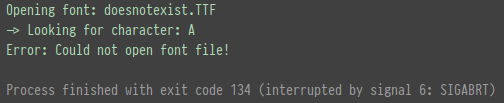
\includegraphics[width=0.9\textwidth]{notfound}
  \caption{\textit{The program rejects invalid or nonexistent files.}}
\end{figure}

\subsection{Objective 3: The system will correctly parse the tables head, cmap, loca, and glyf to read the font.}

Testing this was quite difficult, because just looking at the font file it is often
difficult to determine what the correct outputs of the parser should be. To
remedy this, I took advantage of the fact that freetype, one of the existing
solutions described in the Analysis section, is open source, which meant I could
inspect it's internals. I debugged the freetype library using the same debug
tools above, to check that the values reported by freetype were the same as the
ones that I was parsing. This was a great help during development, where I
couldn't check that the fonts were rendering correctly because the parser and
renderer was not complete.

\subsection{Objective 4: The system will output information about the tables on stdout.}

\begin{figure}[h]
  \centering
  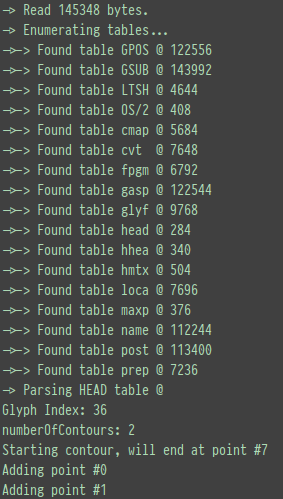
\includegraphics[width=0.2\textwidth]{tables2}
  \caption{\textit{The program outputs various information on the tables on
      stdout for debugging purposes.}}
\end{figure}

\subsection{Objective 5: The parser section of the system will output bezier
  curves that can be sent to the renderer to display the font, or exposed via an
  API for use in some other application.}

This was achieved by the parser system, which outputs the curves needed to then
render the glyph in the rendering section. For example, the curves needed to
render the character `A' are composed of 12 points, as seen in the debug view
below:

\begin{center}
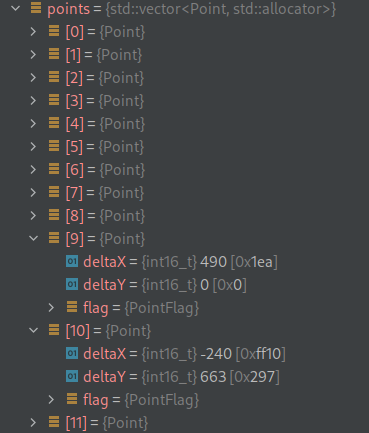
\includegraphics[width=0.4\textwidth]{pointss}
\end{center}

Testing that these points are correct was done by putting them into the
renderer, and observing that the correct glyph was displayed:

\begin{center}

\includegraphics[width=.45\textwidth]{sample1}
\end{center}

\chapter{Evaluation}


\end{document}
